\documentclass[10pt,a4paper]{article}
\usepackage[a4paper,bindingoffset=0.2in,%
            left=1in,right=1in,top=1in,bottom=1in,%
            footskip=.25in]{geometry}

\usepackage[utf8x]{inputenc}
\usepackage[spanish]{babel}

\usepackage{mathtools}
\usepackage{amsmath}
\usepackage{amsfonts}
\usepackage{amssymb}

\usepackage{xcolor}
\usepackage{listingsutf8}
\usepackage{booktabs}
\usepackage{hyperref}
\usepackage{multirow}

\usepackage{caption}
\usepackage{subcaption}

\usepackage{float}
\usepackage[]{algorithmicx}
\usepackage[noend]{algpseudocode}

\usepackage{graphicx}
\usepackage{tikz}
\usepackage{relsize}
\usepackage{epstopdf}

\DeclarePairedDelimiter{\ceil}{\lceil}{\rceil}

% set the default code style
\lstset{
    frame=tb, % draw a frame at the top and bottom of the code block
    tabsize=4, % tab space width
    showstringspaces=false, % don't mark spaces in strings
    numbers=left, % display line numbers on the left
    commentstyle=\color{green}, % comment color
    keywordstyle=\color{blue}, % keyword color
    stringstyle=\color{red} % string color
}

% mathy stuff
\newtheorem{theorem}{Theorem}[section]
\newtheorem{lemma}[theorem]{Lemma}
\newtheorem{proposition}[theorem]{Proposición}
\newtheorem{corollary}[theorem]{Corollary}

\newenvironment{proof}[1][Demostración]{\begin{trivlist}
\item[\hskip \labelsep {\bfseries #1}]}{\end{trivlist}}
\newenvironment{definition}[1][Definición]{\begin{trivlist}
\item[\hskip \labelsep {\bfseries #1}]}{\end{trivlist}}
\newenvironment{example}[1][Example]{\begin{trivlist}
\item[\hskip \labelsep {\bfseries #1}]}{\end{trivlist}}
\newenvironment{remark}[1][Remark]{\begin{trivlist}
\item[\hskip \labelsep {\bfseries #1}]}{\end{trivlist}}

\newcommand{\qed}{\nobreak \ifvmode \relax \else
      \ifdim\lastskip<1.5em \hskip-\lastskip
      \hskip1.5em plus0em minus0.5em \fi \nobreak
      \vrule height0.75em width0.5em depth0.25em\fi}

\title{Aprendizaje Automatico \\ Trabajo Práctico 2 \\ Un jugador inteligente de Cuatro En Línea }

%\newcommand{\order}[1]{$\mathcal{O}(#1)$}

\begin{document}

%% cover page

\maketitle

\bigskip

\begin{table}[h]
\centering
\begin{tabular}{|l l l l|}
\hline
Integrante       & \multicolumn{1}{c}{LU}     & Correo electrónico              & Carrera \\ \hline
Martin Baigorria & \multicolumn{1}{c}{575/14} & martinbaigorria@gmail.com & Computación (Licenciatura) \\
Damián Furman & \multicolumn{1}{c}{936/11}& damian.a.furman@gmail.com & Computación (Licenciatura)\\
Germán Abrevaya & \multicolumn{1}{c}{-} & germanabrevaya@gmail.com & Física (Doctorado)\\ \hline
\end{tabular}
\end{table}

\vfill

\begin{center}
\textbf{Reservado para la cátedra}
\end{center}
\begin{table}[h]
\centering
\begin{tabular}{|l|l|l|}
\hline
Instancia       & Docente & Nota \\ \hline
Primera entrega &         &      \\ \hline
Segunda entrega &         &      \\ \hline
\end{tabular}
\end{table}

\newpage
\tableofcontents
\newpage

% end cover page

\section{Introducción}

El objetivo del presente trabajo practico es estudiar como se comporta un agente que utiliza la técnica de aprendizaje QLearning a partir del juego Cuatro En Línea. Modelaremos el juego, discutiremos detalles de implementación y analizaremos como los diferentes hiperparametros del algoritmo afectan el rendimiento de un jugador, como la tasa de aprendizaje $\alpha$, la inicialización del tablero, el parámetro $\epsilon$ que define la probabilidad de que el agente haga un movimiento meramente aleatorio y los epochs de entrenamiento para ver como progresivamente el jugador va mejorando su performance. Haremos diferentes benchmarks comparando el rendimiento de jugadores que utilizan QLearning y jugadores que toman decisiones de forma aleatoria.

\section{Implementación}

La implementación del juego y los diferentes algoritmos fue realizada en Python 2.7. Antes de remarcar los detalles que nos parecieron relevantes, a continuación mostramos el pseudocódigo del algoritmo QLearning:

\begin{algorithmic}
\Repeat \: para cada episodio
	\State Inicializar s
	\Repeat (para cada paso del episodio):
		\State Repetir (para cada paso del episodio):
		\State Elegir a en s según una política basada en Q
		\State Ejecutar la acción a, observar r, s'
		\State Q(s,a) $\leftarrow$ Q(s,a) + $\alpha$ [r + $\gamma$ $max_{a'}$ Q(s',a') - Q(s,a)]
		\State s $\leftarrow$ s'
	\Until{s sea terminal}
\Until termina el juego
\end{algorithmic}

Un detalle que nos pareció relevante mencionar es el uso de memoria. A medida que el algoritmo va descubriendo nuevos estados, debe poder identificarlos en un futuro. Para ello, debe guardar algún tipo de representación del estado en memoria y el valor de Q para determinada acción asociada. En el caso del Cuatro En Linea, sea $w$ el ancho del tablero y $h$ la altura del tablero. La cantidad de estados asociados al juego estará acotada superiormente por $3^{w*h}$, dado que cada casillero puede tener una ficha de algún jugador, o estar vacío. Esto nos da una indicación de que la memoria va a ser importante, dado que su uso parece ser exponencial en el tamano del tablero. La cantidad de estados en juegos no finitos o hasta con mas estados posibles puede agravar mas aun este problema. En nuestro caso particular, dado que el juego es finito, decidimos representarlos simplemente como la conversión a string de una lista de listas. Debido a que en los tableros que consideramos para realizar este trabajo (hasta 10x10) nunca nos excedimos de los 16GB de RAM disponibles que teníamos, no buscamos una representación mejor del tablero. En otros contextos puede llegar a ser sumamente relevante una representación mas compacta que explote de forma óptima la jerarquía de memoria y también evite el swapping a disco. Aquí también hay un trade off en el sentido que una representación compacta puede llegar a tener la desventaja de llevar mas tiempo de computo para calcular.

Otro detalle que consideramos al momento de experimentar fue la elección del learning rate $\alpha$. Muchas veces queremos evaluar el rendimiento de un algoritmo dado cierta cantidad de epochs en un escenario estático de Q, donde la performance esta influenciada solo por el valor actual de Q y el el azar. Por esta razón al determinar la tasa de partidas ganadas dado un Q fijo, hicimos que el jugador juegue 500 partidas con $\alpha = 0$ para suspender el entrenamiento para luego restaurar el valor de $\alpha$ original.

Cual es el jugador que comienza a jugar también es una variable relevante. Si un jugador se entrena jugando siempre primero, su entrenamiento no sera relevante al momento de jugar segundo dado que el conjunto de estados alcanzables arrancando segundo no son alcanzables arrancando primero. Un hack interesante seria unificar la memoria de dos Qlearners, uno que arranque siempre primero, y otro que arranque siempre segundo. De esta forma conjeturamos que entrenar un jugador que se adapte a ambos escenarios seria mas rápido que entrenar uno solo que alterna si arranca o va segundo de forma aleatoria.

\pagebreak

\section{Experimentación}

\subsection{QLearning vs Random Player}

Una vez implementado el algoritmo de Q Learning, decidimos testearlo en un tablero de 5$\times$5 haciéndolo jugar contra un jugador que elige movidas \textit{random} de entre aquellas disponibles. De esta manera podemos observar si el jugador se comporta efectivamente de manera inteligente y si mejora a partir de su experiencia. Elegimos para nuestro jugador inteligente un porcentaje de jugadas aleatorias (epsilon) del 20\%, un \textit{learning rate} (alpha) de 0.8, un \textit{discount factor} (gamma) de 0.9, recompensa por ganar de 1, recompensa por perder de -1, y por empatar 0.5.

La siguiente figura muestra la tasa de victorias para cada jugador (Qlearner en azul y Random en verde) a medida que aumenta la cantidad de partidas de entrenamiento del algoritmo. Cada punto de estos gráficos están distanciados por 1000 partidas de entrenamiento y calculados promediando 500 partidas en las que solo se jugaba sin entrenar. En un principio la tasa de victorias de ambos jugadores fluctúa alrededor de 0.45, y luego a partir de las 30.000 partidas comienza a diverger. A partir de las 1000.000 partidas la tasa de victorias comienza a converger en forma asintótica a 0.82 el Qlearner, y 0.15 el Random aproximadamente. Esto pone en evidencia un significativo aprendizaje por parte del algoritmo de QLearning.

\iffalse
\begin{figure}[H]
\centering
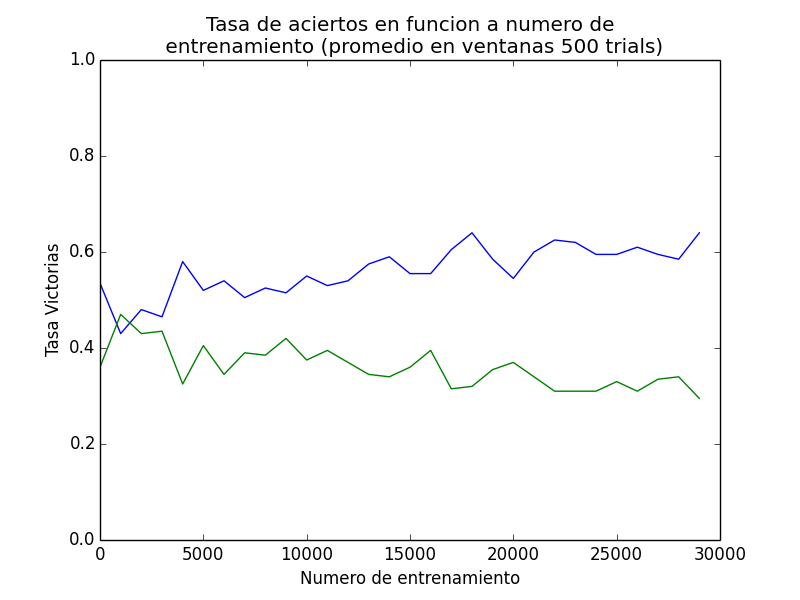
\includegraphics[scale=0.5]{images/random_vs_qlearning_30000.png}
\caption{Random (verde) vs QLearning (azul). Tasa de aciertos en función al numero de epochs de entrenamiento, con el promedio de victorias en ventanas de 500 trials en un tablero de 5x5. Qlearner: $\epsilon$: 0.2, $\alpha$: 0.8, $\gamma$: 0.9.}
\end{figure}

\begin{figure}[H]
\centering
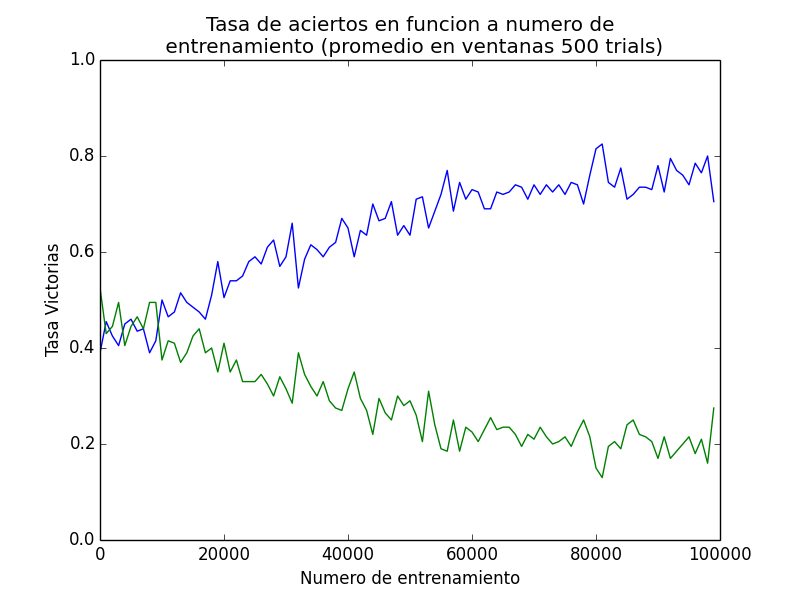
\includegraphics[scale=0.5]{images/random_vs_qlearning_100000.png}
\caption{Random (verde) vs QLearning (azul). Tasa de aciertos en función al numero de epochs de entrenamiento, con el promedio de victorias en ventanas de 500 trials en un tablero de 5x5. Qlearner: $\epsilon$: 0.2, $\alpha$: 0.8, $\gamma$: 0.9.}
\end{figure}
\fi

\begin{figure}[H]
\centering
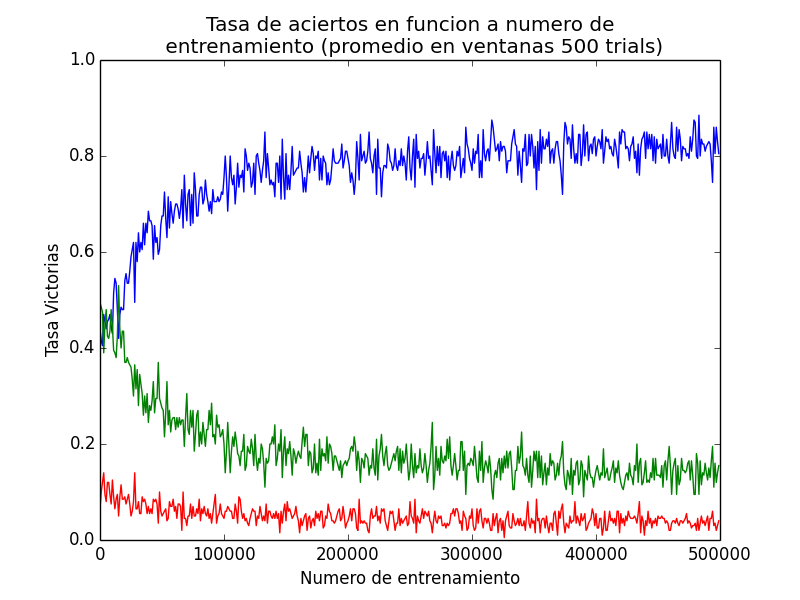
\includegraphics[scale=0.6]{images/q_vs_random_500_with_ties.png}
\caption{Random (verde) vs QLearning (azul). Empates en rojo. Tasa de aciertos en función al numero de epochs de entrenamiento, con el promedio de victorias en ventanas de 500 trials en un tablero de 5x5. Hiperparametros del Qlearner: $\epsilon$: 0.2, $\alpha$: 0.8, $\gamma$: 0.9.}
\end{figure}

A su vez, junto con el resultado correspondiente a las quinientas mil partidas jugadas, incluimos también la tasa promedio de partidas empatadas (curva roja). Puede observarse en el gráfico que la tasa de empates presenta un comportamiento decreciente a medida que aumenta la cantidad de entrenamientos, que comienza en valores cercanos a 0.1 y termina en valores cercanos a 0.05. Una posible explicación de que las fluctuaciones iniciales de las tasas de victorias no sean alrededor de 0.5 (y el asociado comienzo no nulo de la tasa de empates) es que son más las formas que existen de empatar que de ganar y es por esto que jugado aleatoriamente (jugador \emph{Random} y \emph{Q Learner} teniendo muy poco entrenamiento) es más probable que el partido resulte empatado. Es decir, jugando al azar es más probable empatar, al menos para este tamaños de tablero.

\pagebreak

\subsection{QLearning vs QLearning}

Luego de experimentar con un jugador random, decidimos experimentar con dos jugadores entrenados de la misma manera, con iguales hiperparámetros ídenticos a los de la Sección anterior), que partiesen de las mismas condiciones. Ambos jugadores tienen la misma probabilidad de arrancar jugando. Queremos observar así cómo se comporta nuestro algoritmo de aprendizaje ante otro jugador que también mejora con el paso del tiempo. Partimos de la hipótesis de que luego de un período en el cual alguno de los jugadores podría sacarle cierta ventaja al otro, deberían tender a estabilizarse en la medida en que completen su entrenamiento debido a que éste se realiza, para ambos, en las mismas condiciones. A su vez, esperábamos que el \textit{ratio} de los empates aumentase en la medida que ambos jugadores mejoraran ya que el que Qlearner además de aprender a ganar aprende a evitar perder.

\begin{figure}[H]
\centering
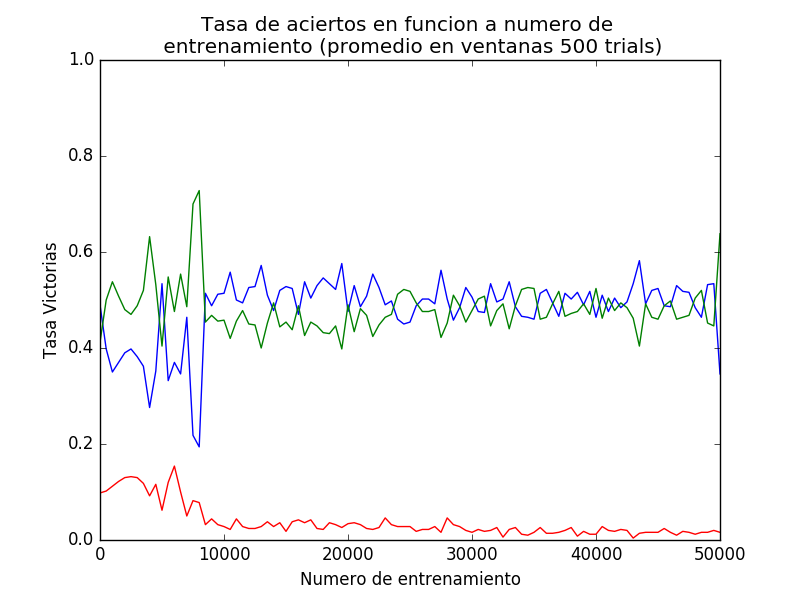
\includegraphics[scale=0.6]{images/QlearnervsQlearner50000.png}
\caption{QLearning vs QLearning. Empates en rojo. Tasa de aciertos en función al numero de epochs de entrenamiento, con el promedio de victorias en ventanas de 500 trials en un tablero de 5x5. Hiperparametros de ambos Qlearners: $\epsilon$: 0.2, $\alpha$: 0.8, $\gamma$: 0.9.}
\end{figure}

Los resultados que se observaron fueron en contra de nuestra intuición. Como muestra la figura anterior, la cantidad de empates es muy baja y comenzamos a sospechar que algo no estaba bien. Sin embargo, luego conjeturamos que en realidad el jugador que arranca el juego siempre tiene una estrategia ganadora. Para comenzar a testear esta hipótesis, cambiamos la forma en que se entrenaban los jugadores para que sistemáticamente uno siempre arrancara primero.

\begin{figure}[H]
\centering
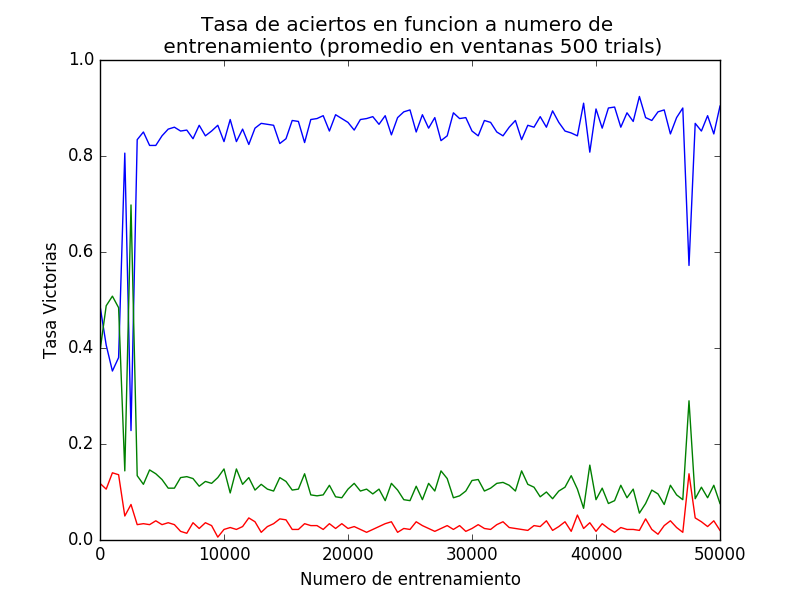
\includegraphics[scale=0.6]{images/qvsq_arranca.png}
\caption{QLearning vs QLearning. Empates en rojo. El jugador azul es el que siempre comienza. Tasa de aciertos en función al numero de epochs de entrenamiento, con el promedio de victorias en ventanas de 500 trials en un tablero de 5x5. Hiperparametros de ambios Qlearners: $\epsilon$: 0.2, $\alpha$: 0.8, $\gamma$: 0.9.}
\end{figure}

Esto fue evidencia en favor de la hipótesis, aunque no es evidencia conclusiva. Efectivamente el jugador que arranca parece tener ventaja. Sin embargo, hay otros factores como la elección de hiperparametros que pueden estar interfiriendo en nuestro experimento. Es posible también que los agentes solo aprendieron a atacar pero nunca a defenderse. Intentamos cambiar los rewards del tablero, dándole un reward de -100 al caso en el que el agente pierde y los resultados fueron muy similares. Tambien observamos que el agente que siempre iba segundo se defendía sumamente bien, evitando en general perder de forma trivial de ser posible (horizontal, vertical y en diagonal).

Esta demostrado que este juego tiene una estrategia ganadora para el jugador que comienza. La prueba formal excede el scope de este trabajo, pero puede encontrarse en la bibliografía [1],[2]. Esto nos da la pauta de la relevancia de la elección de hiperparametros y estrategias de temperatura y velocidad con las que se enfría el sistema. En teoría se podría lograr hasta un 15\% de mejora para el jugador que arranca de esta manera.

\subsection{Variaciones sobre Épsilon}

El hiperpárametro \emph{épsilon} determina la probabilidad de que un jugador decida hacer una jugada aleatoria, en vez de seguir la estrategia `óptima' dada por el valor de su función Q. Este hiperpárametro le permite al jugador explorar el espacio de jugadas. En una primera instancia explorar es deseable para poder aprender. Sin embargo, a medida que el jugador tiene más experiencia, se podría esperar que su Q comience a converger a su Q óptimo. Es decir que tras cierta cantidad de entrenamientos dejaría de ser conveniente tener un alto grado de aleatoriedad en sus decisiones para poder hacer más uso de lo ya aprendido. Realizamos experimentaciones haciendo competir a un jugador \textit{Qlearner} con uno \textit{Random} variando el hiperparámetro \textit{épsilon} pero manteniendo fijo el resto con los valores usados en las secciones anteriores. Cabe destacar que el \emph{épsilon} que variamos es el usa \emph{QLearning} en los entrenamientos, sin embargo siempre en las partidas de `testing', de las que se sacan los datos para confeccionar los gráficos, se el \emph{Qlearner} está configurado para usar un \emph{épsilon} nulo, determinando que siempre elija según lo aprendido y nunca al azar.\\

\begin{figure}[H]
\makebox[\textwidth][c]{
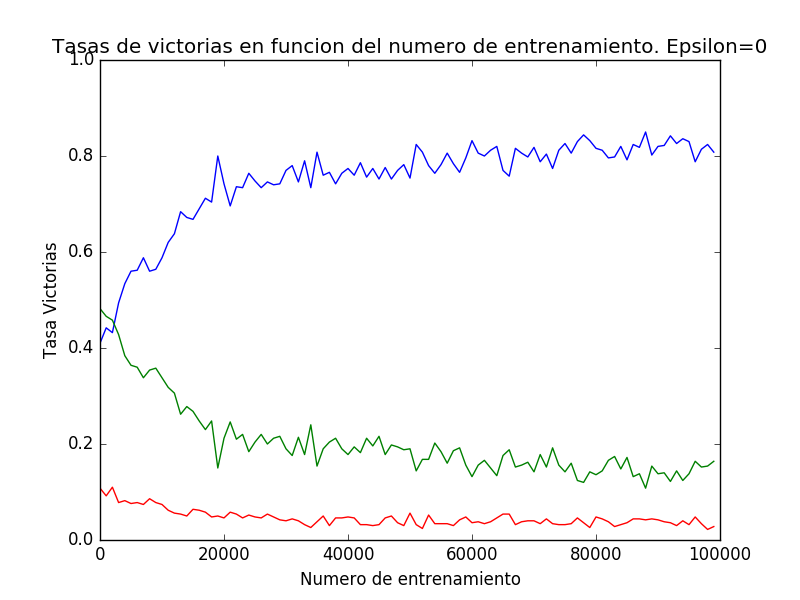
\includegraphics[scale=0.4]{images/q_vs_random_epsilon_0.png}
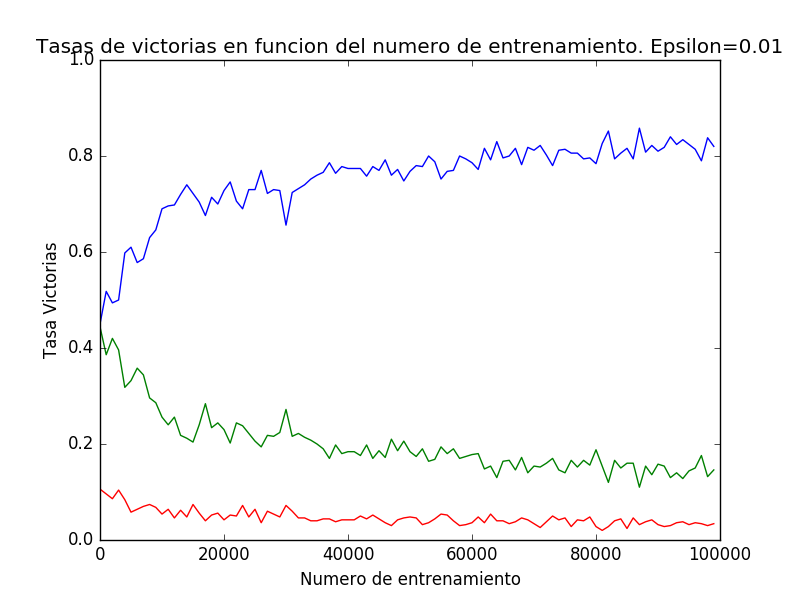
\includegraphics[scale=0.4]{images/q_vs_random_epsilon_0_01.png}
}
\end{figure}

\begin{figure}[H]
\makebox[\textwidth][c]{
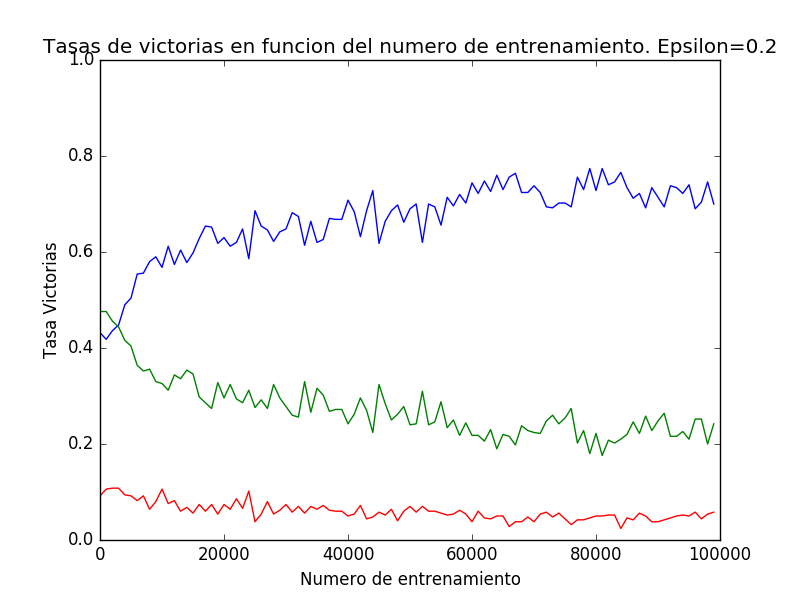
\includegraphics[scale=0.4]{images/q_vs_random_epsilon_0_2.png}
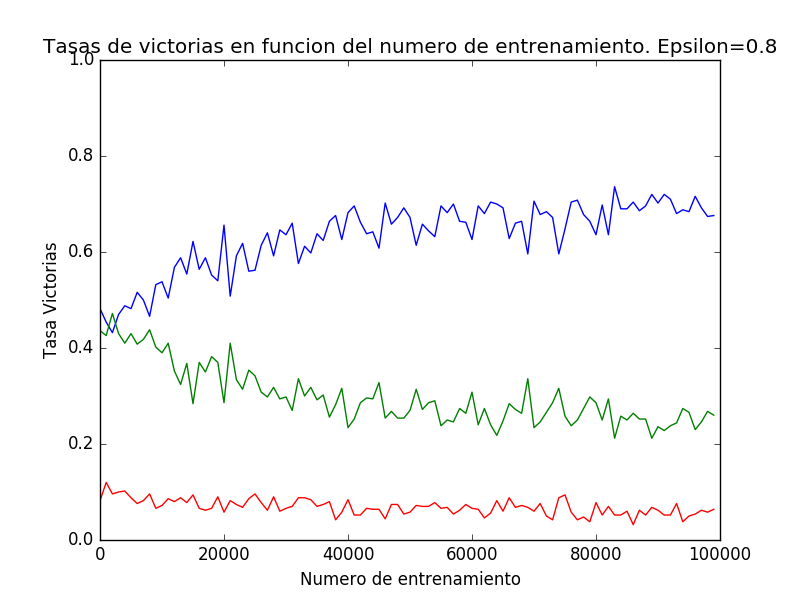
\includegraphics[scale=0.4]{images/q_vs_random_epsilon_0_8.png}
}
\end{figure}

\begin{figure}[H]
\makebox[\textwidth][c]{
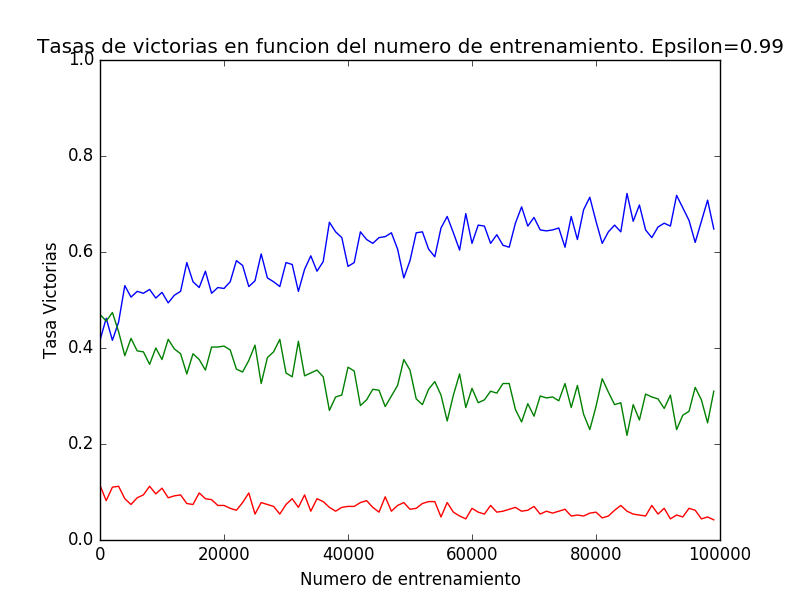
\includegraphics[scale=0.4]{images/q_vs_random_epsilon_0_99.png}
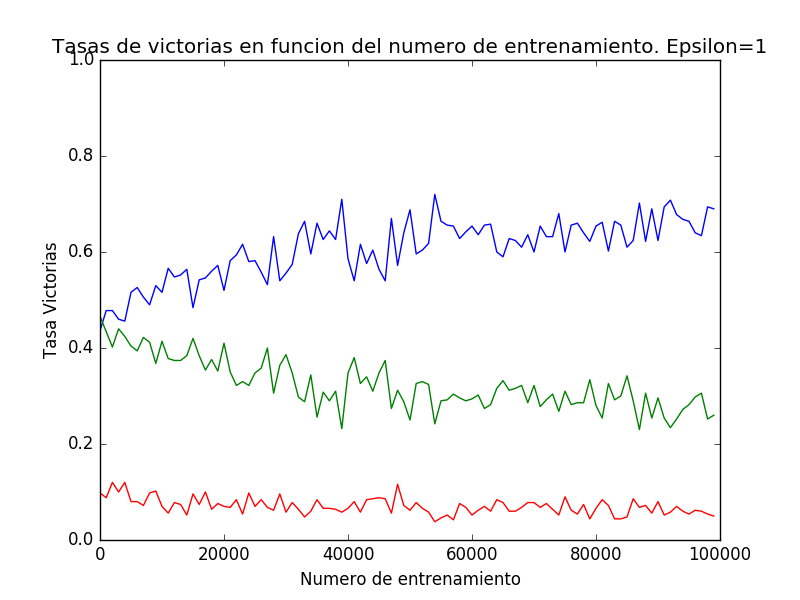
\includegraphics[scale=0.4]{images/q_vs_random_epsilon_1.png}
}
\end{figure}

\begin{figure}[H]
\caption{QLearning (azul) vs Random (verde). Empates en rojo. Tasa de aciertos en función al numero de epochs de entrenamiento, con el promedio de victorias en ventanas de 500 trials en un tablero de 5x5. Hiperparametros del Qlearner: $\alpha$: 0.8, $\gamma$: 0.9, con $\epsilon$ variando de forma creciente de izquierda a derecha, de arriba a abajo. Los épsilon utilizados en orden son: 0, 0.01, 0.2, 0.8, 0.99, 1.}
\end{figure}

Como se puede apreciar en estas figuras, entrenando con valores de \emph{épsilon} 0 y 0,01 se alcanzaron tasas de victorias más altas que para valores mayores. Mientras que a medida que aumentaba \emph{épsilon}, es decir la probabilidad de elegir una jugada al azar, el aprendizaje fue más lento, requiriendo más entrenamiento para obtener estadísticas de victorias similares. Asimismo, se observa que al aumentar \emph{épsilon} aumenta la varianza de los resultados de las partidas, ilustrado en el ruido de las curvas graficadas.

\subsection{Variaciones sobre Alpha}
El hiperparámetro \textit{alpha} o \textit{learning rate} establece con qué rapidez una información `nueva' reemplazará a la información previa. Representa el impacto que una experiencia contraria a aprendizajes anteriores puede generar. Mientras que un \textit{learning rate} igual a 0 indica que nuestro jugador no aprende nada, un \textit{learning rate} igual a 1 indica que sólo tomamos en consideración la última experiencia realizada en cuanto al valor de una jugada en un determinado tablero. Las experiencias previas fueron realizadas con un \textit{learning rate} con valor 0.8. A continuación estudiamos los efectos de modificar este hiperparámetro asignándole valores menores.

En primer lugar, observamos el resultado de entrenar nuestro jugador \textit{Q Learning} con parámetro \textit{alpha} igual a 0.2. Un valor bajo de \textit{alpha} retrasa las tendencia que se expresa con el aprendizaje. El algoritmo aprende más lento, entonces lo que aprende tarda más en manifestarse. Si observamos el \textit{ratio} de victorias luego de cien mil partidas jugadas observamos que las del jugador \textit{Q Learning} y del jugador \textit{Random} están mucho más cercanos entre si que en los hallados en las figuras de la sección 2.1, con $alpha$ = 0.8. Incluso al ver el resultado luego de doscientas mil partidas vemos que si bien ya se manifiesta una tendencia cercana al 80\% de victorias para el \textit{Q Learning}, aún no alcanza este valor, lo que sí sucede con mayor claridad en los ejemplos de la sección 2.1.

\begin{figure}[H]
\makebox[\textwidth][c]{
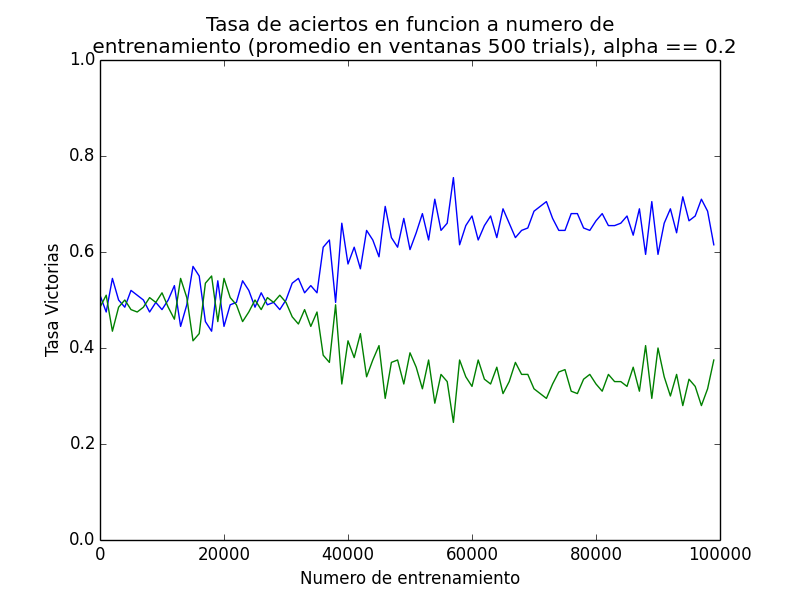
\includegraphics[scale=0.4]{images/q_vs_random_alpha_0_2.png}
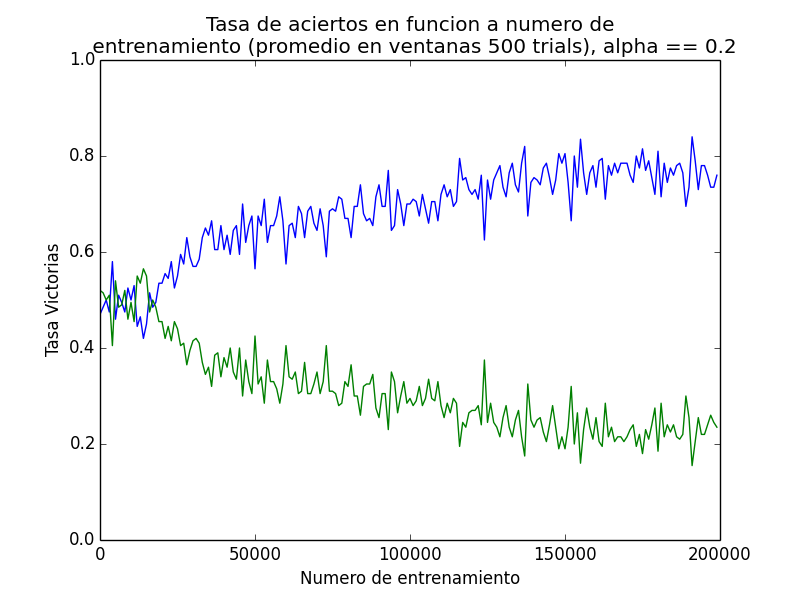
\includegraphics[scale=0.4]{images/q_vs_random_alpha_0_2_200.png}
}
\caption{QLearning (azul) vs Random (verde). Empates en rojo. Tasa de aciertos en función al numero de epochs de entrenamiento, con el promedio de victorias en ventanas de 500 trials en un tablero de 5x5. Hiperparametros del Qlearner: $\epsilon$: 0.2, $\alpha$: 0.2, $\gamma$: 0.9.}
\end{figure}

Por otro lado, para los \textit{alphas} grandes (iguales a 1), un aprendizaje en una coordenada cercana a donde ya habíamos aprendido algo sobreescribe el resto de los aprendizajes. En consecuencia, estamos aprendiendo todo nuevamente, una y otra vez. La naturaleza del juego, además, puede generar tableros en los que la victoria de uno u otro jugador pueda depender de una sóla jugada de cada uno. Es decir que en el espacio de estados una situación victoriosa pueda darse `al lado' de una situación de derrota. Esto puede servir como ejemplo de lo que, según entendemos, no logra captar un aprendizaje con un parámetro alpha igual a 1. En consecuencia, obtenemos una situación curiosa en la que un jugador \textit{Q Learning} no logra superar a un jugador \textit{random}.\footnote{Vale aclarar que este experimento fue ejecutado cinco veces, todas con resultados similares.}

\begin{figure}[H]
\centering
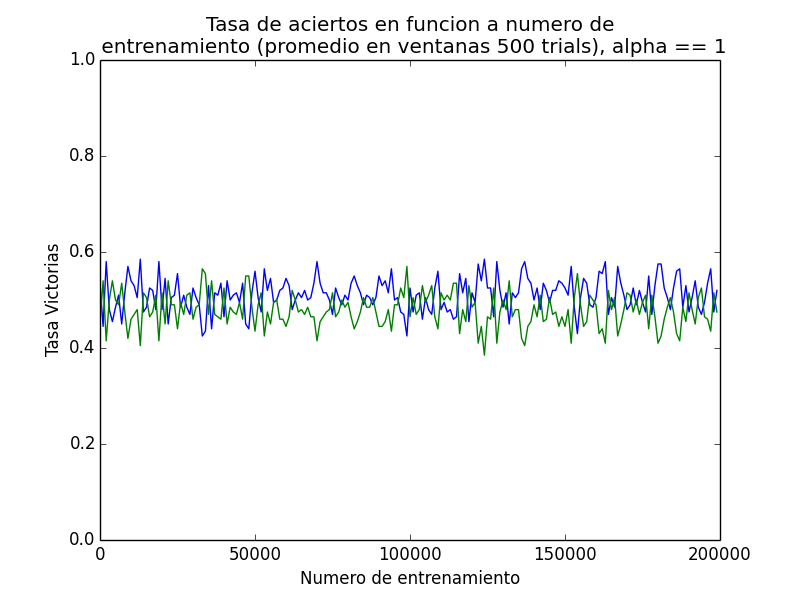
\includegraphics[scale=0.5]{images/q_vs_random_alpha_1_200_v2.png}
\caption{QLearning (azul) vs Random (verde). Empates en rojo. Tasa de aciertos en función al numero de epochs de entrenamiento, con el promedio de victorias en ventanas de 500 trials en un tablero de 5x5. Hiperparametros del Qlearner: $\epsilon$: 0.2, $\alpha$: 1, $\gamma$: 0.9.}
\end{figure}

\subsection{Variaciones sobre Gamma}

El hiperparámetro \textit{gamma} representa el \textit{discount factor}. Cuanto más bajo sea este parámetro, menos se esparcirá una recompensa positiva o negativa hacia los cuadrantes cercanos y, por lo tanto, menor será la influencia que tenga sobre estos. Si el discount factor es, por ejemplo, 0, el algoritmo de aprendizaje sólo será capaz de reconocer que se encuentra cerca de la victoria cuando esté a una jugada de distancia. Si por el contrario, el discount factor es 1, cada victoria se propagará sin limites hacia todos los posibles casilleros, lo cual no permitiría distinguir entre un tablero entre el que se puede ganar en una jugada de uno en el que se puede ganar en 20. A continuación observamos los resultados obtenidos luego de entrenar a nuestro jugador \textit{Q Learner} contra un jugador \textit{Random} durante doscientas mil partidas con tres valores distintos de \emph{gamma}: 0, 0.4 y 1.\\

\begin{figure}[H]
\makebox[\textwidth][c]{
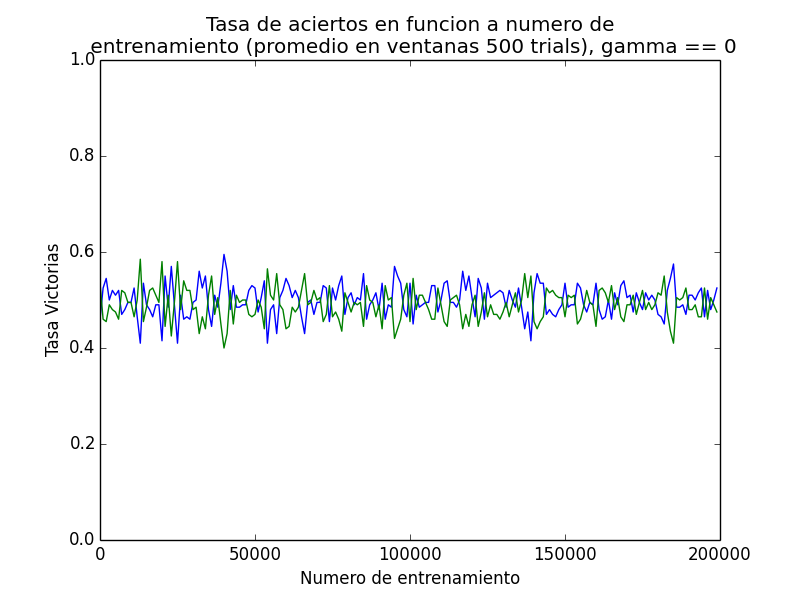
\includegraphics[scale=0.4]{images/q_vs_random_gamma_0_200.png}
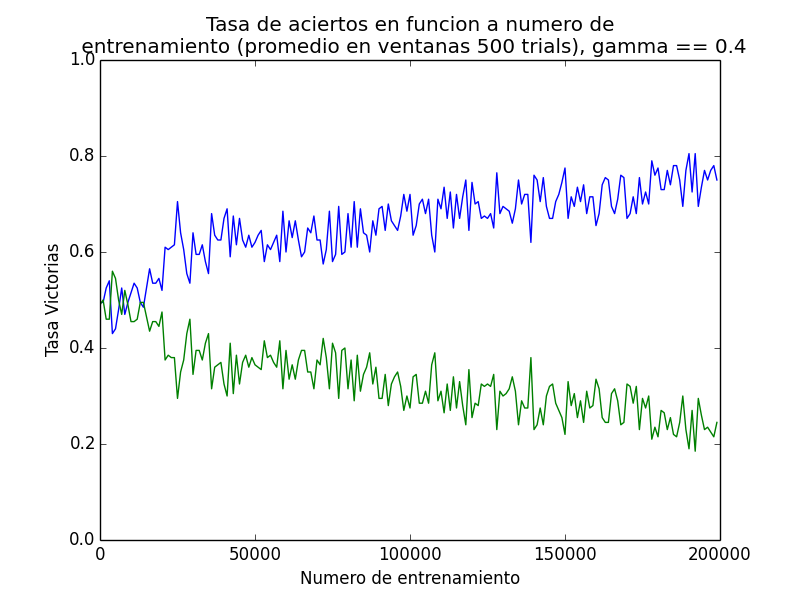
\includegraphics[scale=0.4]{images/q_vs_random_gamma_0_4_200.png}
}
\caption{QLearning (azul) vs Random (verde). Empates en rojo. Tasa de aciertos en función al numero de epochs de entrenamiento, con el promedio de victorias en ventanas de 500 trials en un tablero de 5x5. Hiperparametros del Qlearner: $\epsilon$: 0.2, $\alpha$: 0.8, con $\gamma$ variando de izquierda a derecha: 0, 0.4}
\end{figure}

\pagebreak

Se observa que cuando \textit{gamma} es nulo el \textit{Q Learner} no consigue superar el desempeño de un jugador \textit{Random} al cabo de 200000 juegos de entrenamiento. La extrema localidad en el espacio de estados del aprendizaje hace que éste sea inefectivo. Por otro lado, entre los casos de \emph{gamma} = 1 y \emph{gamma} = 0.4, más allá de demora inicial por parte del primero, no se observan diferencias importantes en las tasas de victorias tras los 200.000 entrenamientos.

\section{Conclusión}

Pudimos ver que a través del algoritmo de QLearning, a pesar de ser relativamente simple y no estar diseñado específicamente para este juego --de hecho sin conocer sus reglas sino únicamente el resultado final y el espacio de estados posibles--, se puede obtener un desempeño considerable. Se alcanzaron tasas de ganancia de 0.82 de un jugador entrenado con QLearning respecto a uno que jugaba al azar. Incluso al jugar un ser humano inexperto en el Cuatro en Línea (como los autores de este trabajo) contra un Qlearner suficientemente entrenado, difícilmente puede llegar a ganar el ser humano.

Uno de los resultados que nos sorprendió fue la aparente existencia de una estrategia ganadora para el jugador que arranca el juego.

Dado que es un juego finito y a un jugador lo único que le importa es ganar, no cuanto tiempo le tome, conjeturamos que lo óptimo es que el factor de descuento utilizado al calcular Q sea 1. En general se usa un factor de descuento menor a 1 en juegos que no son finitos para forzar a que el agente tome una desicion que lleve lo suficientemente rápido hacia una victoria.

Al momento de jugar contra un player \textit{Qlearner}, una vez que ya estaba entrenado en general se lo configuro con un epsilon de 0, para que siempre siga la jugada óptima de acuerdo a su matriz de retornos esperados Q. Por cuestiones de tiempo no fue posible experimentar con estrategias de elección de epsilon para mejorar la velocidad de entrenamiento.

Dado que la dimension de Q es exponencial en el tamano del tablero, muchas veces no es factible recorrer todos los estados del juego. Para tableros chicos, es razonable explorar gran parte del espacio. Caso contrario, uno debe seguir una estrategia un poco mas greedy y limitarse a un subconjunto del espacio. Aquí entra nuevamente el parámetro epsilon. A menor epsilon, se podría decir que nuestro algoritmo es mas greedy.

Otro factor importante que se podría llegar a analizar es el efecto de la inicialización del tablero sobre la velocidad de entrenamiento. En general, para todo este trabajo se inicializaron todos los estados posibles con un payoff de 1, que en general hace que el jugador busque explorar más.

También conjeturamos que los rewards relativos cuando un jugador gana, pierde o empata llevan a que un jugador sea mas o menos agresivo en su juego. El nivel de agresividad de un jugador es difícil de medir, pero podríamos decir que si al jugador solo le importa ganar y no empatar, quizás gane más que si juega contra uno que solo le importa no perder.

\section{Referencias}

[1] Allen, J.D.: A note on the computer solution of connect-four. In: Levy, D.N.L., Beal, D.F. (eds.) Heuristic Programming in Artificial Intelligence, The first Computer Olympiad, pp. 134–135. Ellis Horwood, Chinchester (1989).

[2] Allis, L.V.: A Knowledge-Based Approach to Connect-Four. The game is solved: White wins, Master’s thesis, Vrije Universiteit (1988)

\end{document}